\documentclass[11pt,a4paper]{article}
\usepackage[T1]{fontenc}
\usepackage[utf8]{inputenc}
\usepackage[french]{babel}
\usepackage{booktabs,longtable,array,amsmath}
\usepackage[a4paper,margin=2.4cm]{geometry}
\usepackage{graphicx}
\usepackage[hidelinks]{hyperref}
\usepackage{microtype}
\setlength{\parindent}{0pt}
\setlength{\parskip}{0.55em}

\title{Rapport d'implémentation du modèle M2}
\author{Réplication computationnelle indépendante}
\date{3 juillet 2026}

\begin{document}
\maketitle

\begin{abstract}
M2 a été implémenté comme paquet Python autonome, sans modification des modèles
historiques. Le noyau suit les sept phases du rapport, maintient un carnet nominal
indexé et vérifie les invariants de bilan. Vingt-sept tests couvrent les cas
normaux et limites. Un premier run long a révélé une explosion combinatoire des
fragments de créances ; elle a été corrigée par une fusion par paire exactement
équivalente pour des contrats nominaux perpétuels. Trois baselines de 2000 pas ont
ensuite abouti. Ce rapport décrit le logiciel et ses limites ; les conclusions
statistiques sont réservées au rapport de validation.
\end{abstract}

\tableofcontents

\section{Objectifs et méthode}

L'objectif était d'obtenir une implémentation fidèle, modulaire, reproductible et
auditable avant toute recherche de forme distributionnelle. Le travail a suivi
l'ordre inventaire $\rightarrow$ lecture critique $\rightarrow$ spécification
$\rightarrow$ tests $\rightarrow$ simulations. Tous les nouveaux fichiers sont
isolés sous \texttt{m2\_codex/} afin d'éviter une collision avec un autre agent.

Le générateur aléatoire est local à chaque simulation
(\texttt{numpy.random.Generator(seed)}). Les références entre entités utilisent
des identifiants entiers. La simulation n'a ni capacité de charge, ni mortalité
exogène, ni seuil de population.

\section{Architecture réalisée}

\begin{longtable}{p{0.28\textwidth}p{0.63\textwidth}}
\toprule
Fichier & Rôle \\
\midrule
\endhead
\texttt{src/m2/config.py} & Configuration immuable et validation des domaines. \\
\texttt{entities.py} & État individuel minimal et flux du dernier pas. \\
\texttt{contracts.py} & Contrats, index prêteur/emprunteur, caches de bilans et
fusion exacte par paire. \\
\texttt{market.py} & Taux marginal, cible de capital et matching local. \\
\texttt{bankruptcy.py} & Liquidation, transfert de créances et cascades. \\
\texttt{simulation.py} & Sept phases, service d'intérêts et orchestration. \\
\texttt{metrics.py}, \texttt{storage.py} & Séries, snapshots, schémas CSV/JSON. \\
\texttt{analysis.py}, \texttt{plots.py} & Ajustements, bootstrap par blocs,
diagnostics et figures. \\
\texttt{experiments/m2/} & Baseline, validation, grille, ablations et agrégation
des rapports. \\
\bottomrule
\end{longtable}

\begin{figure}[ht]
\centering
\fbox{\begin{minipage}{0.9\textwidth}\centering
\texttt{M2Config + seed} $\longrightarrow$ \texttt{M2Simulation}\\
$\downarrow$ sept phases et audits $\downarrow$\\
\texttt{StepMetrics + snapshots + events}
$\longrightarrow$ \texttt{analysis.py} $\longrightarrow$ tableaux et figures
\end{minipage}}
\caption{Séparation entre dynamique, persistance et analyse. Les graphiques ne
peuvent pas modifier la trajectoire ni consommer le RNG du modèle.}
\end{figure}

\section{Choix opérationnels explicites}

Le rapport ne définissait pas le service simultané de plusieurs dettes. La
baseline calcule les capacités au début de la phase et répartit un paiement
partiel au prorata des intérêts dus. Cela supprime la priorité arbitraire d'un
ordre de dictionnaire. La variante séquentielle par identifiant est disponible
en ablation.

Une entité marquée en défaut ne participe pas au marché qui précède sa
liquidation. Les faillites sont examinées par identifiant ; une récupération
reçue plus tôt dans la vague peut sauver une insolvabilité non encore défaillante.
Les créances de la faillie sont fractionnées entre ses créanciers admissibles ;
une créance sans repreneur est annulée. Son capital sans créancier est détruit et
mesuré. Toutes ces conventions figurent dans la configuration ou les rapports.

Le cas $w=0$ est traité par la limite sans prêt, plutôt que par un epsilon
dynamique. Les valeurs non finies arrêtent le run. Le critère de faillite reste
strictement $\mathrm{NW}<0$.

\section{Invariants et tests}

La commande de référence est :
\begin{verbatim}
PYTHONPATH=src /home/anatole/jupyter/.venv/bin/python3 \
  -m unittest discover -s tests -v
\end{verbatim}

Les 27 tests passent. Ils couvrent :
\begin{itemize}
  \item naissance, valeur nette, $w=0$, $q=0$, $N=0$ et $N<k$ ;
  \item création/suppression de contrat et cohérence des index ;
  \item conservation du principal et de la valeur nette lors d'un prêt ;
  \item intérêts complets, intérêts partiels prorata et défaut ;
  \item faillite avec ou sans créancier, transfert fractionné et cascade ;
  \item absence de capital négatif et de contrat orphelin ;
  \item reproductibilité par seed et neutralité de la cadence des snapshots ;
  \item données synthétiques exponentielles et Pareto pour l'analyse.
\end{itemize}

Après chaque pas audité, le code vérifie $w\geq0$, les extrémités vivantes,
$q>0$, l'égalité entre total des créances, total des dettes et principal du
carnet, puis l'absence de défaillante après cascade.

\section{Résultat numérique imprévu et correction}

La traduction littérale du transfert prorata a créé 3482 contrats à $t=1200$,
25243 à $t=1300$, 74807 à $t=1400$ et 142766 à $t=1414$. Le premier run long a
été interrompu à 588 Mo de mémoire. Cette croissance provenait du nombre de
fragments, pas de l'encours.

Deux contrats de même paire $(\ell,b)$, de principaux $q_1,q_2$ et taux
$r_1,r_2$, sont désormais remplacés par
\[
q=q_1+q_2,\qquad r=\frac{r_1q_1+r_2q_2}{q_1+q_2}.
\]
Le principal, l'intérêt $rq$, les bilans et les poids prorata sont exactement
conservés. Comme il n'existe ni maturité, ni amortissement, ni dépréciation des
contrats, aucune information dynamique pertinente n'est perdue. Seule la lignée
détaillée des fragments est compressée en compteur de composantes. Après
correction, seed 0 atteint $t=2000$ avec 14096 relations et environ 51 Mo dans la
sonde sans audits continus.

\section{Résultats d'exécution}

Trois runs baseline ont terminé à 2000 pas. Le seed 0 a conservé les audits à
chaque pas ; les seeds 1 et 2 ont effectué l'audit final après passage de la même
suite de tests. Les populations finales sont respectivement 1672, 1680 et 1677 ;
les nombres de faillites cumulées 18242, 18379 et 18281. Aucun invariant n'a été
violé.

\begin{figure}[ht]
\centering
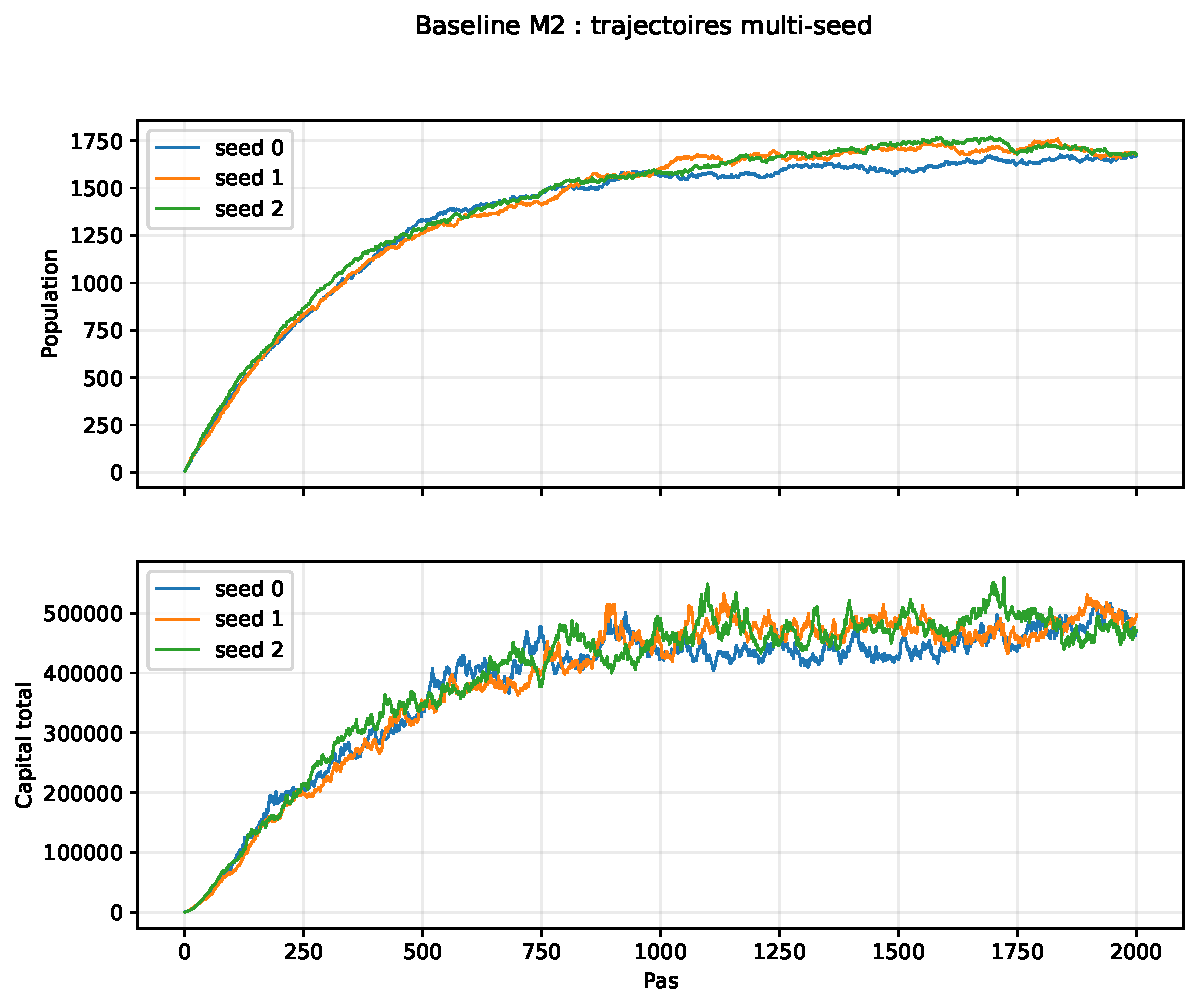
\includegraphics[width=0.95\textwidth]{../04_validation_report/figures/baseline_multiseed.pdf}
\caption{Trajectoires des trois baselines. Le plateau visuel doit être confronté
aux pentes résiduelles, discutées dans le rapport de validation.}
\end{figure}

Les sorties comprennent \texttt{run.json}, \texttt{timeseries.csv}, 40 snapshots
CSV par run, figures PNG/PDF, \texttt{analysis.json} et tableaux de validation.
Le schéma inclut capital, valeur nette, créances, dettes, âge, extraction,
intérêts reçus/payés et revenus brut/net.

\section{Limites et risques restants}

La liquidation séquentielle reste dépendante de l'ordre lorsque deux faillites
peuvent se sauver mutuellement ; une liquidation simultanée n'a pas encore été
implémentée. Le lot de faillites par pas mélange plusieurs déclencheurs initiaux :
ce n'est pas une avalanche causale isolée. Le carnet agrégé ne conserve pas la
généalogie complète des fragments. Enfin, le coût croît avec le nombre de paires
actives ; aucun seuil de troncature n'a été introduit, par prudence scientifique.

Le venv ne contient pas \texttt{pytest}; la suite utilise \texttt{unittest}, ce
qui satisfait l'exigence d'une commande unique sans dépendance supplémentaire.

\section{Prochaines expériences}

Il faut prolonger certains runs au-delà de 2000 pas pour tester le plateau,
implémenter la liquidation simultanée, isoler des avalanches causales, répéter la
grille sur plusieurs seeds et tester l'invariance de temps en divisant $\delta$.
L'intégration au \texttt{simulation\_lab} n'est pas nécessaire à la validation du
noyau et a volontairement été différée.

\section{Conclusion}

L'implémentation est fidèle aux mécanismes explicites de M2 et rend visibles ses
conventions manquantes. Elle est testée, reproductible et capable d'exécuter les
runs longs sans capacité de charge ni réglage numérique de la richesse. La
correction du carnet est une équivalence comptable démontrable, pas une
modification économique. Le logiciel est donc utilisable pour juger le modèle ;
il ne préjuge pas du verdict statistique, qui est largement négatif sur le corps
exponentiel et plus ambigu sur la queue.

\end{document}
